% CVPR 2027 submission, version 1.1 (2026-10-12). Teacher/student framing; devil's advocate terminology; teacher-uncertainty result.
\documentclass[10pt,twocolumn,letterpaper]{article}
\usepackage[review]{cvpr}
\usepackage{graphicx,booktabs,amsmath,amssymb,multirow,xcolor}
\usepackage{cuted,caption}
\definecolor{cvprblue}{rgb}{0.21,0.49,0.74}
\usepackage[pagebackref,breaklinks,colorlinks,allcolors=cvprblue]{hyperref}
\newcommand{\pend}[1]{{\color{red}[#1]}}
\def\paperID{*****}\def\confName{CVPR}\def\confYear{2027}
\title{The Teaching Round: Supplementary Material}
\author{Anonymous}
\renewcommand{\thetable}{S\arabic{table}}\renewcommand{\thefigure}{S\arabic{figure}}
\begin{document}
\maketitle
\section{Selection audit of VLM zoom}
\begin{table}[t]\centering\small
\caption{\textbf{VLM zoom transitions} relative to the global-view answer (95\% bootstrap CI). Adversarial = best-of all grid tiles (white-box option scores); realized = the model's own grounding zoom.}\label{tab:vlm}
\setlength{\tabcolsep}{2.5pt}
\resizebox{\linewidth}{!}{\begin{tabular}{@{}lccc@{}}\toprule
 & V* Qwen2.5 & V* Qwen3 & HR-4K Qwen2.5\\\midrule
global-view acc & .665 & .691 & .600\\
full high-res acc & .707 & .743 & .590\\\midrule
\multicolumn{4}{@{}l}{\emph{correct$\to$wrong} (among global-correct)}\\
\ adversarial tile & .457 {\tiny[.37,.55]} & .568 {\tiny[.49,.65]} & .383 {\tiny[.30,.48]}\\
\ random tile (expected) & .092 & .130 & .132\\
\ best-of natural zooms & .087 & .073 & .192\\
\ realized own zoom & .063 & .058 & .080\\\midrule
\multicolumn{4}{@{}l}{\emph{wrong$\to$correct} (among global-wrong)}\\
\ realized own zoom & .590 & .675 & .359\\
\ some tile & .969 & .949 & .700\\\bottomrule
\end{tabular}}\end{table}

Tab.~\ref{tab:vlm}: the VLM's answer depends strongly on the crop. The deployed zoom is net helpful (it repairs 36--68\% of wrong answers and breaks 6--8\% of correct ones), and plausible alternative zooms are only mildly harmful (7--19\%). The risk is concentrated in adversarial choice: one authentic tile, shown together with the global view, breaks 38--57\% of correct answers, 3--5$\times$ the random-tile rate. The same evidence dependence that makes zoom useful (some tile repairs 70--97\% of wrong answers) makes it steerable.

\section{Systems that ignore the selected evidence}
\begin{table}[t]\centering\small
\caption{\textbf{DeepEyes-7B crop-service substitution} (V*, 191 questions; every substitution replaces every crop the agent requests). Transitions relative to the agent's own rollout. Crop-necessary: questions Qwen2.5-VL answers wrongly from the global view but correctly with the GT tile (n=46).}\label{tab:deepeyes}
\setlength{\tabcolsep}{3pt}
\begin{tabular}{@{}lcc@{}}\toprule
overview given to the agent & full-res & 768$^2$\\\midrule
native accuracy (tool used on 100\%) & .832 & .681\\
GT crop: accuracy & .838 & .707\\
adversarial crop: correct$\to$wrong & .025 & .015\\
random crop: correct$\to$wrong & .006 & .015\\
blank crop: correct$\to$wrong & .013 & .030\\
crop from another image: correct$\to$wrong & .006 & .030\\
valid-box adversary: correct$\to$wrong & .006 & .007\\\midrule
crop-necessary: native & .696 & .239\\
crop-necessary: GT crop & .696 & .283\\\bottomrule
\end{tabular}\end{table}

DeepEyes~\cite{zheng2025deepeyes} calls its zoom tool on every question, but its answers barely depend on what the tool returns (Tab.~\ref{tab:deepeyes}). Replacing every returned crop with the ground-truth region raises accuracy by at most 2.6 points; adversarial, random, blank, and other-image crops all change at most 3\% of correct answers. On crop-necessary questions with a $768^2$ overview, where the answer is not resolvable from the overview, the agent stays at 24\% and the ground-truth crop lifts it only to 28\%. Transcripts assert that ``the zoom-in confirms'' the answer for crops that do not contain the object. This agent is robust to selection attacks because it does not use the selected evidence, a third regime distinct from robust evidence use, and consistent with MED~\cite{med2026}.

\begin{table}[t]\centering\small
\caption{\textbf{SlideChat on SlideBench-VQA-BCNB} (200 questions per task; controls on 100). Accuracy / balanced accuracy. Full: deployed patch sequence; adversarial: 2 of 16 regions chosen to favor a wrong option; text only: no visual tokens; other slide: a random other slide's full sequence. Majority: always answering the most frequent option.}\label{tab:slidechat}
\resizebox{\linewidth}{!}{\begin{tabular}{lcccccc}\toprule
Task & reported & full & adversarial & text only & other slide & majority\\\midrule
Tumor (3-way) & .894 & .870 / .33 & .870 / .33 & .880 / .33 & .870 / .33 & .885 / .33\\
ER & .791 & .765 / .53 & .760 / .53 & .750 / .52 & .750 / .50 & .785 / .50\\
PR & .703 & .690 / .59 & .665 / .58 & .640 / .56 & .660 / .57 & .725 / .50\\
HER2 & .768 & .780 / .70 & .790 / .69 & .790 / .67 & .800 / .67 & .735 / .50\\\bottomrule
\end{tabular}}
\end{table}
\paragraph{A released slide-level VLM.} We ran the same audit on SlideChat~\cite{slidechat} (CONCH features, LongNet slide encoder, Qwen2.5-7B) with its official stage-2 weights on SlideBench-VQA-BCNB. Our full-slide accuracies reproduce the reported ones within 2.5 points (Tab.~\ref{tab:slidechat}), but every selector, including an adversary choosing 2 of 16 regions, leaves accuracy unchanged, and so do removing the slide entirely or substituting another patient's slide. The reported accuracies sit at the majority-class rate (balanced accuracy .33--.70) and the model's per-region answer probabilities vary by about 0.01 within a slide. This is the tool-insensitivity regime at the slide level: the model cannot be steered by evidence selection because its answers do not depend on the evidence. A teaching round with SlideChat as the teacher is therefore uninformative here (balanced accuracy .30--.70 across all conditions), and we do not report it as a defense result.

\begin{figure}[t]\centering
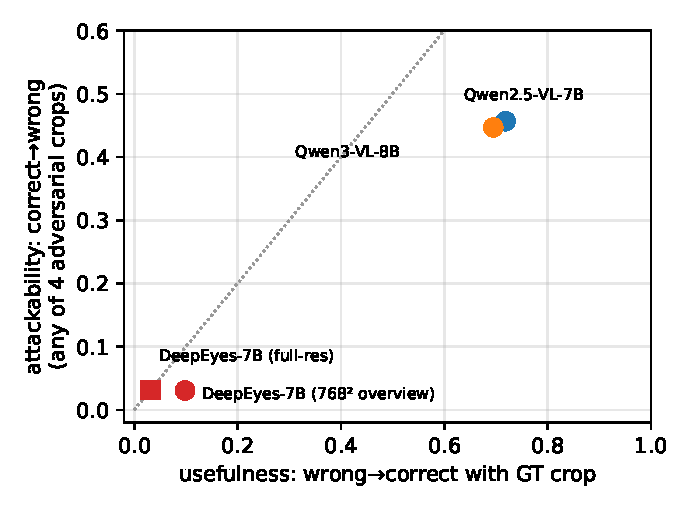
\includegraphics[width=0.92\linewidth]{figs/fig_useful_attack.pdf}
\caption{\textbf{Usefulness and attackability move together} (V*). x: wrong$\to$correct when the GT crop is supplied; y: correct$\to$wrong under any of the \emph{same} four crops chosen with a Qwen2.5-VL surrogate (for Qwen3-VL and DeepEyes this is a black-box transfer attack). Evidence-dependent zoom is both useful and steerable; DeepEyes is neither.}\label{fig:useful}
\end{figure}


{\small\bibliographystyle{ieeenat_fullname}\bibliography{refs}}
\end{document}
